\chapter{Results}
This section will present the results of the measurements with ZnTe and GaP as emitter crystals.
Calculations will be made to determine the electricfield strength of the produced $\si{\tera\hertz}$ radiation aswell as the Power of said radiation.
Futher a comparission between the different spectras of ZnTe and GaP will be shown and the efficiency in producing radiation will be discussed.

\section{Zinc telluride}
For this measurments a $\SI{1}{\milli\meter}$ thick ZnTe crystal is used as the emitter.
Another $\SI{1}{\milli\meter}$ thick ZnTe crystal is used as the detector.
At this point it should be said, that the Znte crystal that is used as the emitter has a burn mark on it.
The burned crystal can be seen in figure \ref{fig:ZnTe_burned}.
Obviously the burned part of the crystal negatively effects efficiency of $\si{\tera\hertz}$ production.
Which is why the part of the laser with the highest power is not focused on the burned part.
Still some of the laser hits the burned part of the crystal crystal.
\\\\
To get an understanding of the data the first figure that should be looked at is the time resolved EOS data.
For this the lock-in Amplifier output is plotted against the time delay between pump and probe beam.
The figure \ref{ZnTe:2_11_30} shows the resulting plot.
This measurement is taken with a pump power of $\SI{135.0}{\milli\W}$, which is the highest pump power that is used.
The typicall trend of a $\si{\tera\hertz}$ pulse can clearly be seen.
Befor the pulse starts the signal is balanced at $X(V)=0$.
\begin{figure}
    \centering
    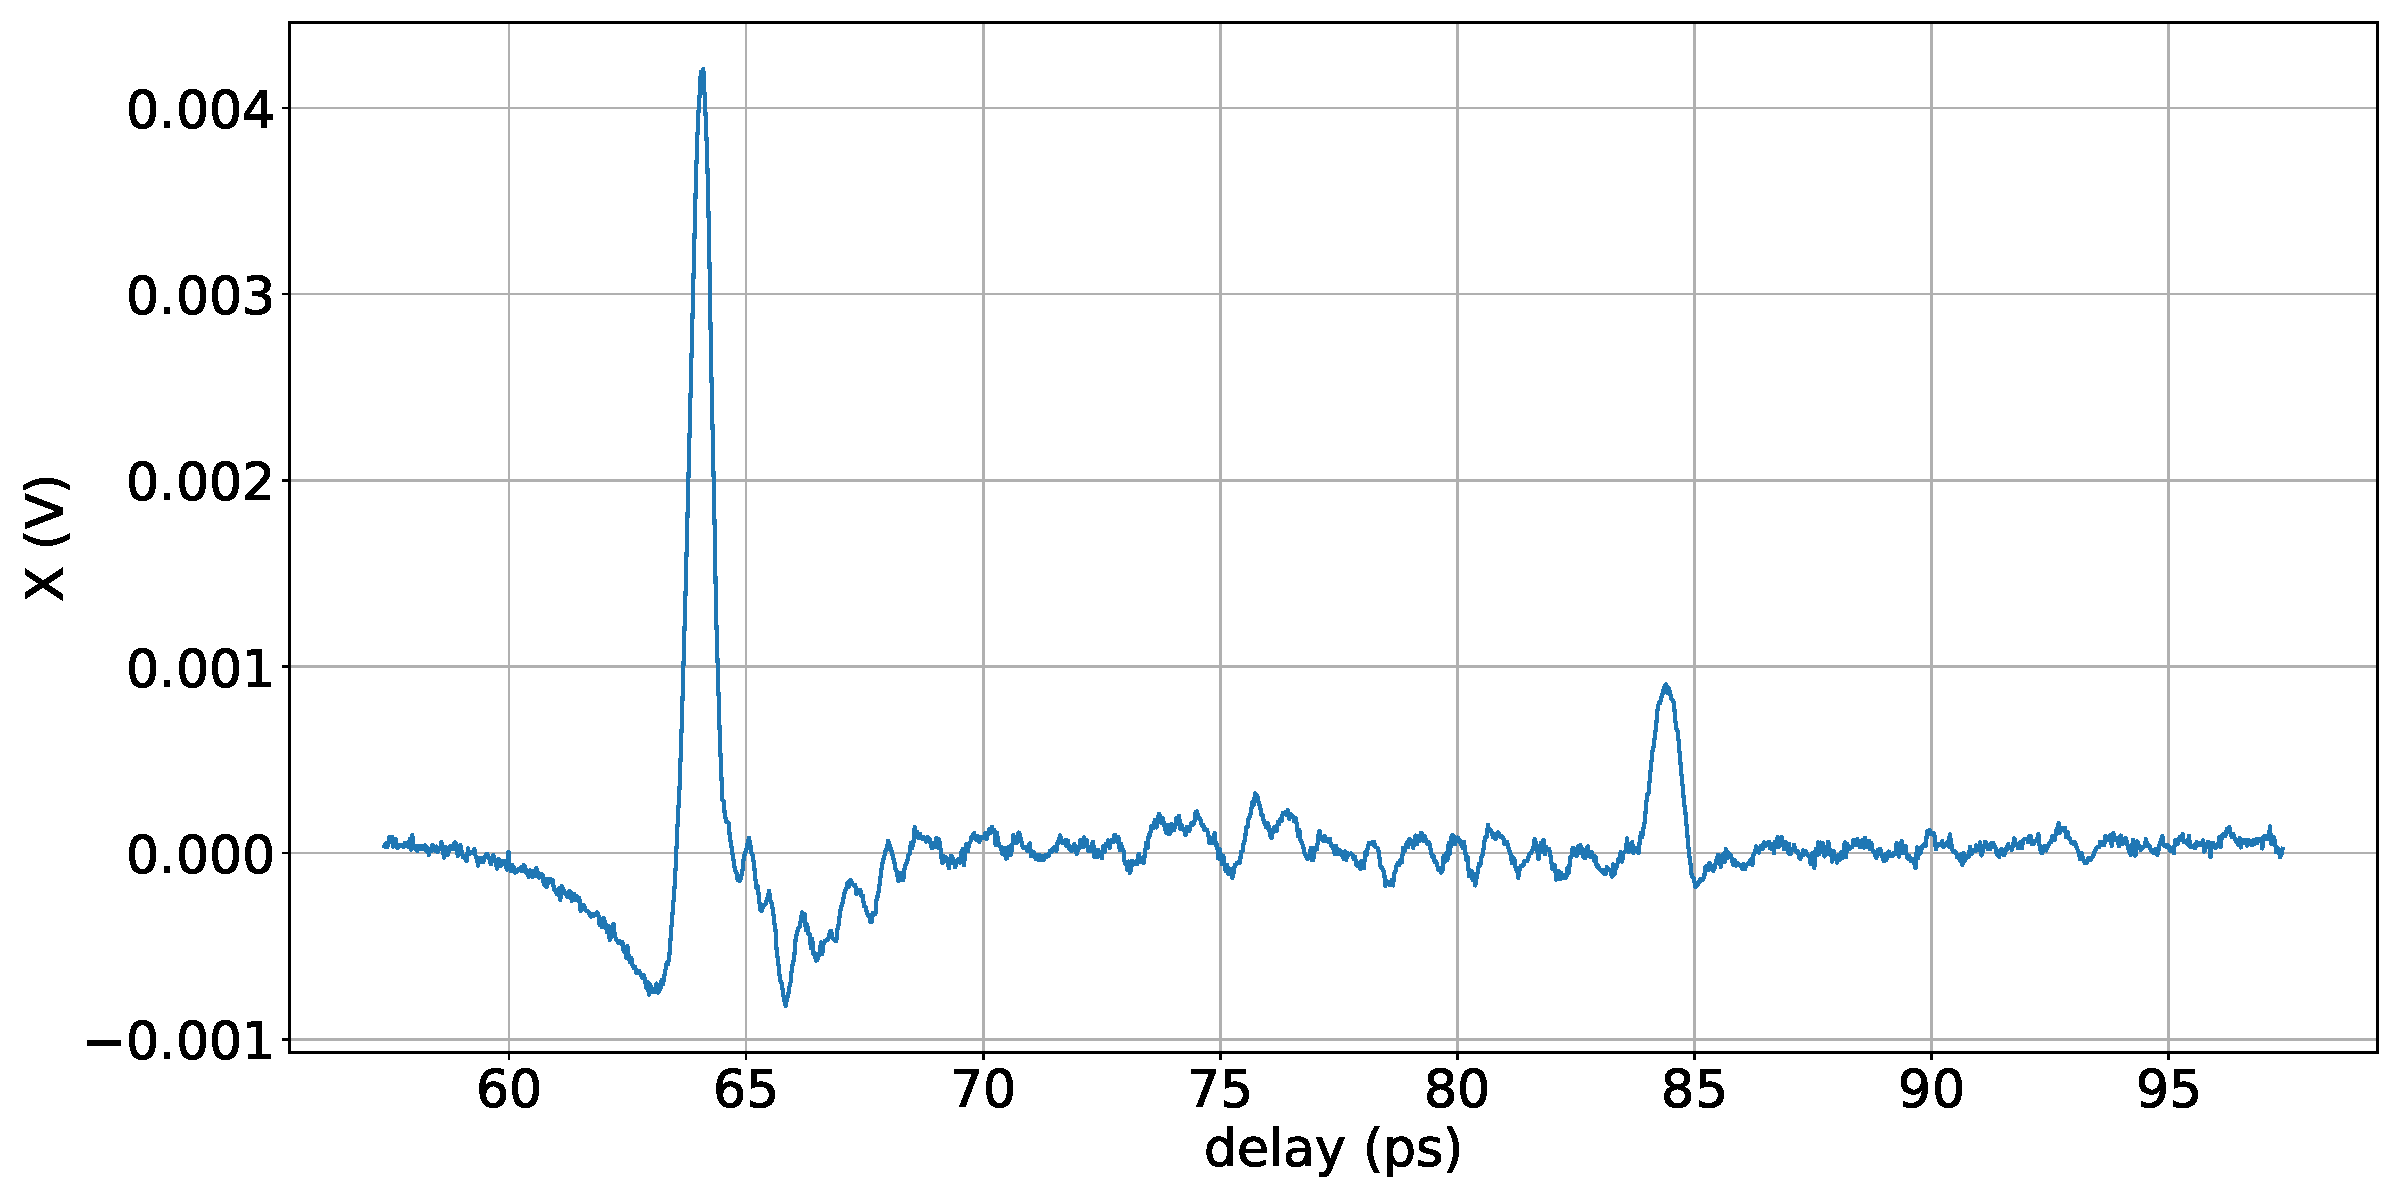
\includegraphics[width=0.5\textwidth]{Plots/2_11_30_20normalX.pdf}
    \caption{The $\si{\tera\hertz}$ pulse, that is measured by EOS, with a pump power of $\SI{135.0}{\milli\W}$.
    The EOS signal is plotted against the delay in $\si{\pico\seconds}$.
    A post pulse can be seen at a delay of $\SI{84}{\pico\seconds}$.}
    \label{ZnTe:2_11_30_20_signal}
\end{figure}
\\
At a delay of about $\SI{58}{\pico\seconds}$ the pulse starts, which manifests in a an increasingly negativ $X(V)$ value.
After about $\SI{5}{\pico\seconds}$ after the start the minimum is reached and the lock-in Amplifier output increases drastically up to a value of $\SI{0.00420669}{\V}$.
Here the maximum of the plot is reached, which corresponses to the maximum $\si{\tera\hertz}$ electricfield strength inside the detector crystal.
After the maximum the signal drops almost to zero.
\\
From this point on there are some oszillations, but no major features are visible. %are those oszialltions acuatlly caused by water?
Up until a delay of $\SI{84}{\pico\seconds}$, where the post pulse starts.
The post pulse is caused by refelections of the $\si{\tera\hertz}$ pulse inside the crystal.
Which is why the post pulse is just an echo of the intial pulse and thus alters the signal in a negativ way.
For futher calculations the data that is taken up until the post pulse will be used, but not the post pulse.
\\\\
\FloatBarrier
To confirm that the pulse that is shown in figure \ref{ZnTe:2_11_30_20_signal} actually corresponses to a $\si{\tera\hertz}$ pulse a Fourier-Transformation of the data is calculated. %Do I need to mention FFT in theory?
Because the Fourier-Transformation is done numerically the FFT function of the python package scipy \cite{scipy} is used.
The resulting Fourierspectrum is shown in figure \ref{fig:2_11_30_20_fft}.
The Spectrum is also plotted against a logarithmic x-axis, which gives the plot in figure \ref{fig:2_11_30_20_fft_log}.
With this it is easy to confirm that the produced radiation actually lies in the $\si{\tera\hertz}$ regime.
Most of the radiation that is produced has a frequenzy between $0.3-1.1\,\si{\tera\hertz}$, but radiation with even higher $\si{\tera\hertz}$ frequencies are produced aswell.
\begin{figure}%
    \begin{subfigure}{0.48\textwidth}%
        \centering%
        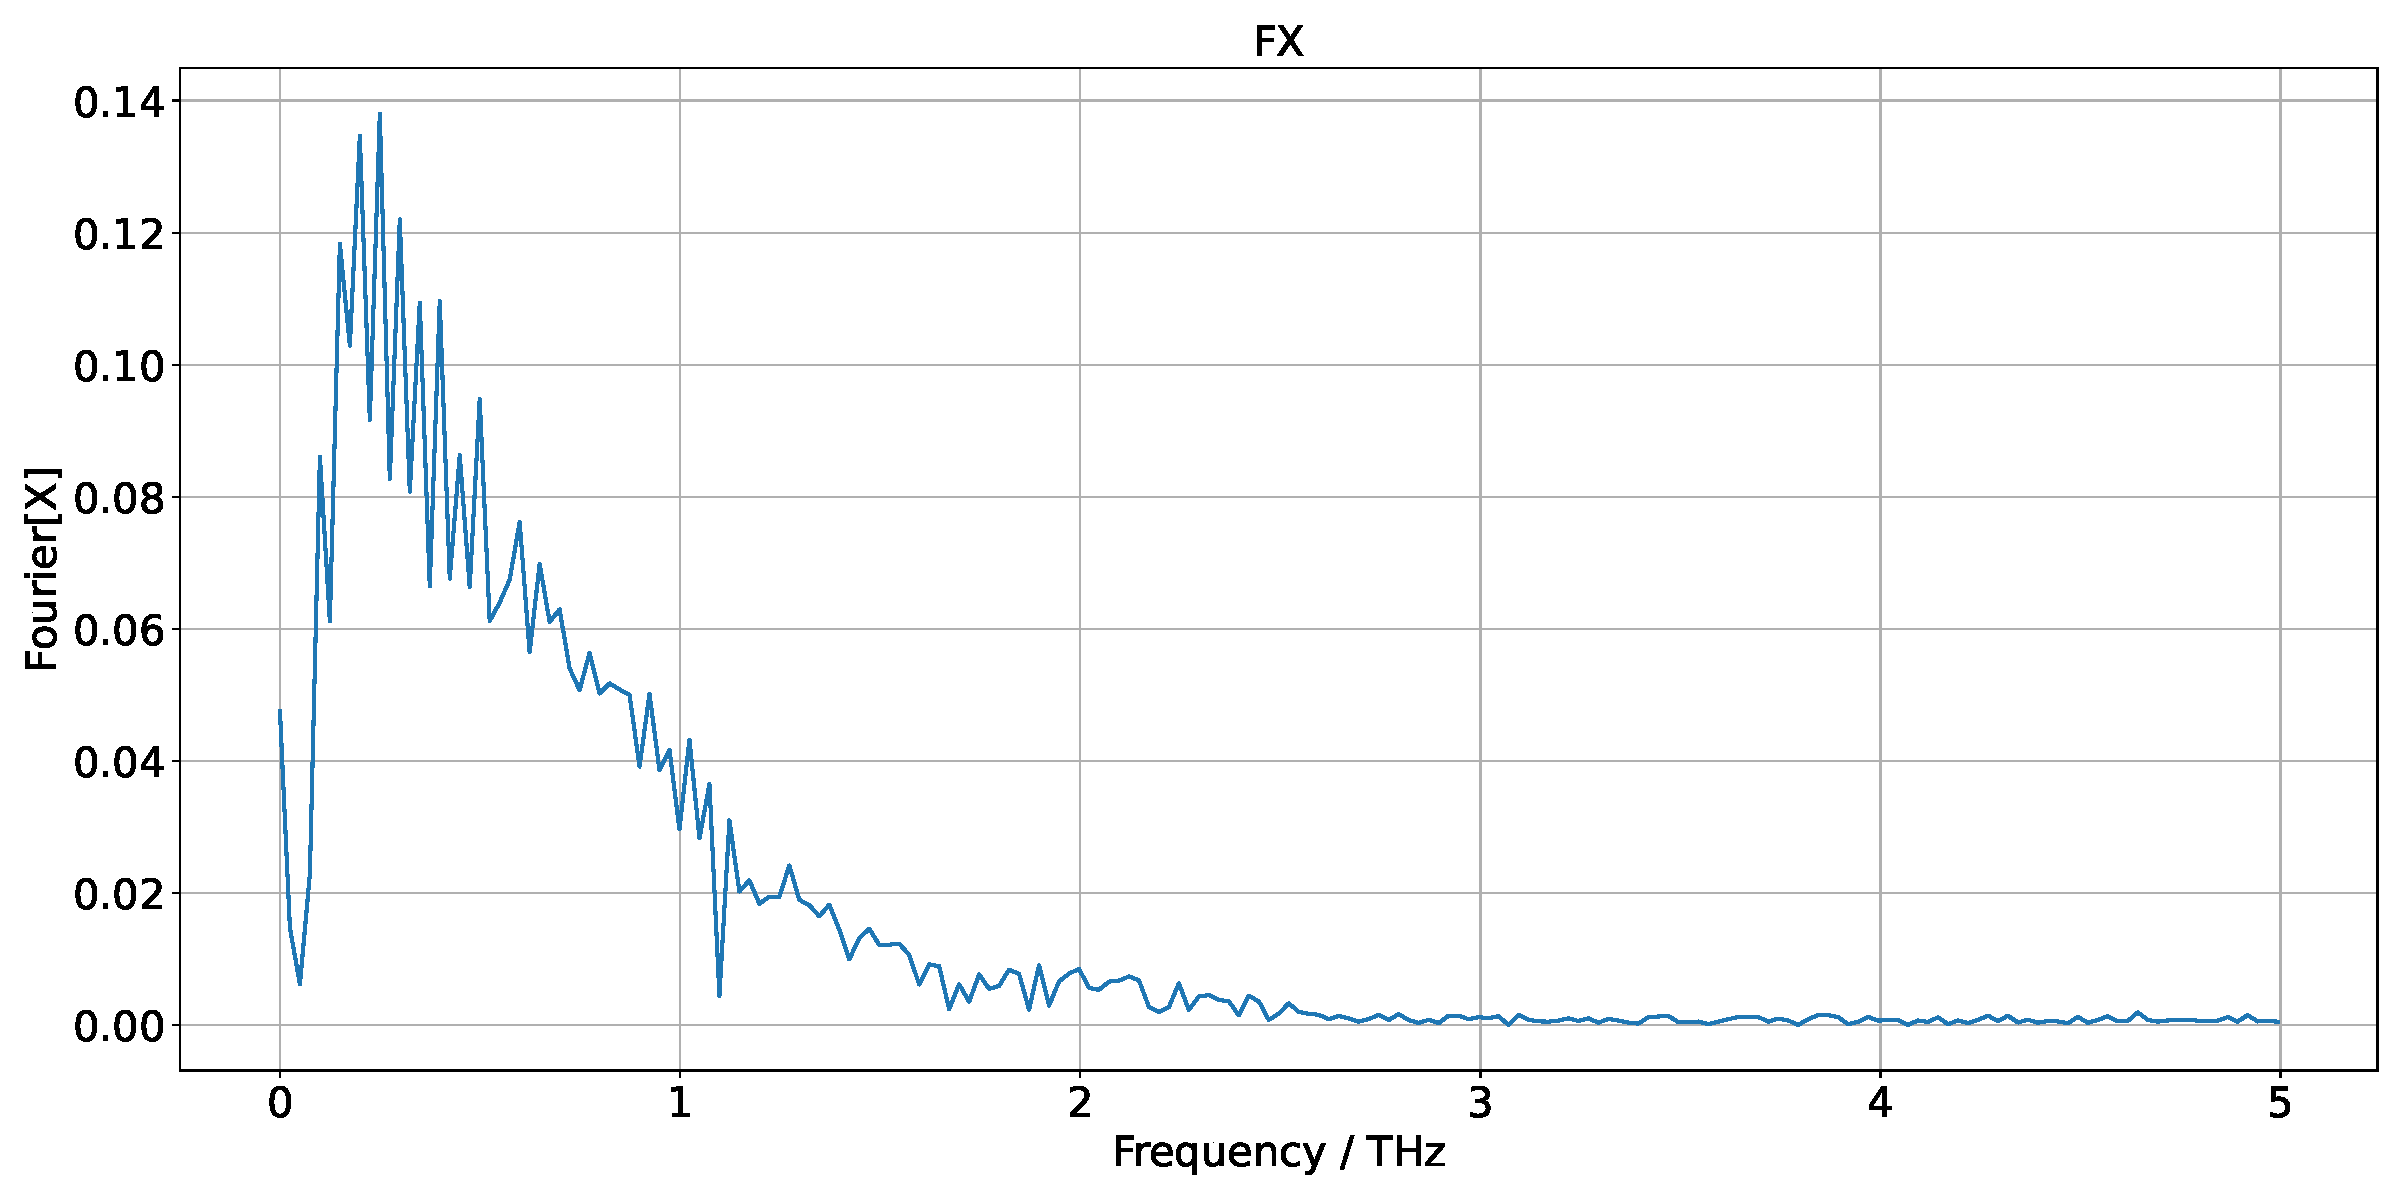
\includegraphics[height=0.75cm]{Plots/2_11_30_20normalFX.pdf}%
        \caption{PeP-Logo.}%
        \label{fig:pep2}%
        \end{subfigure}%
    \hfill% Fills available space in the center -> space between figures
        \begin{subfigure}{0.48\textwidth}%
        \centering%
        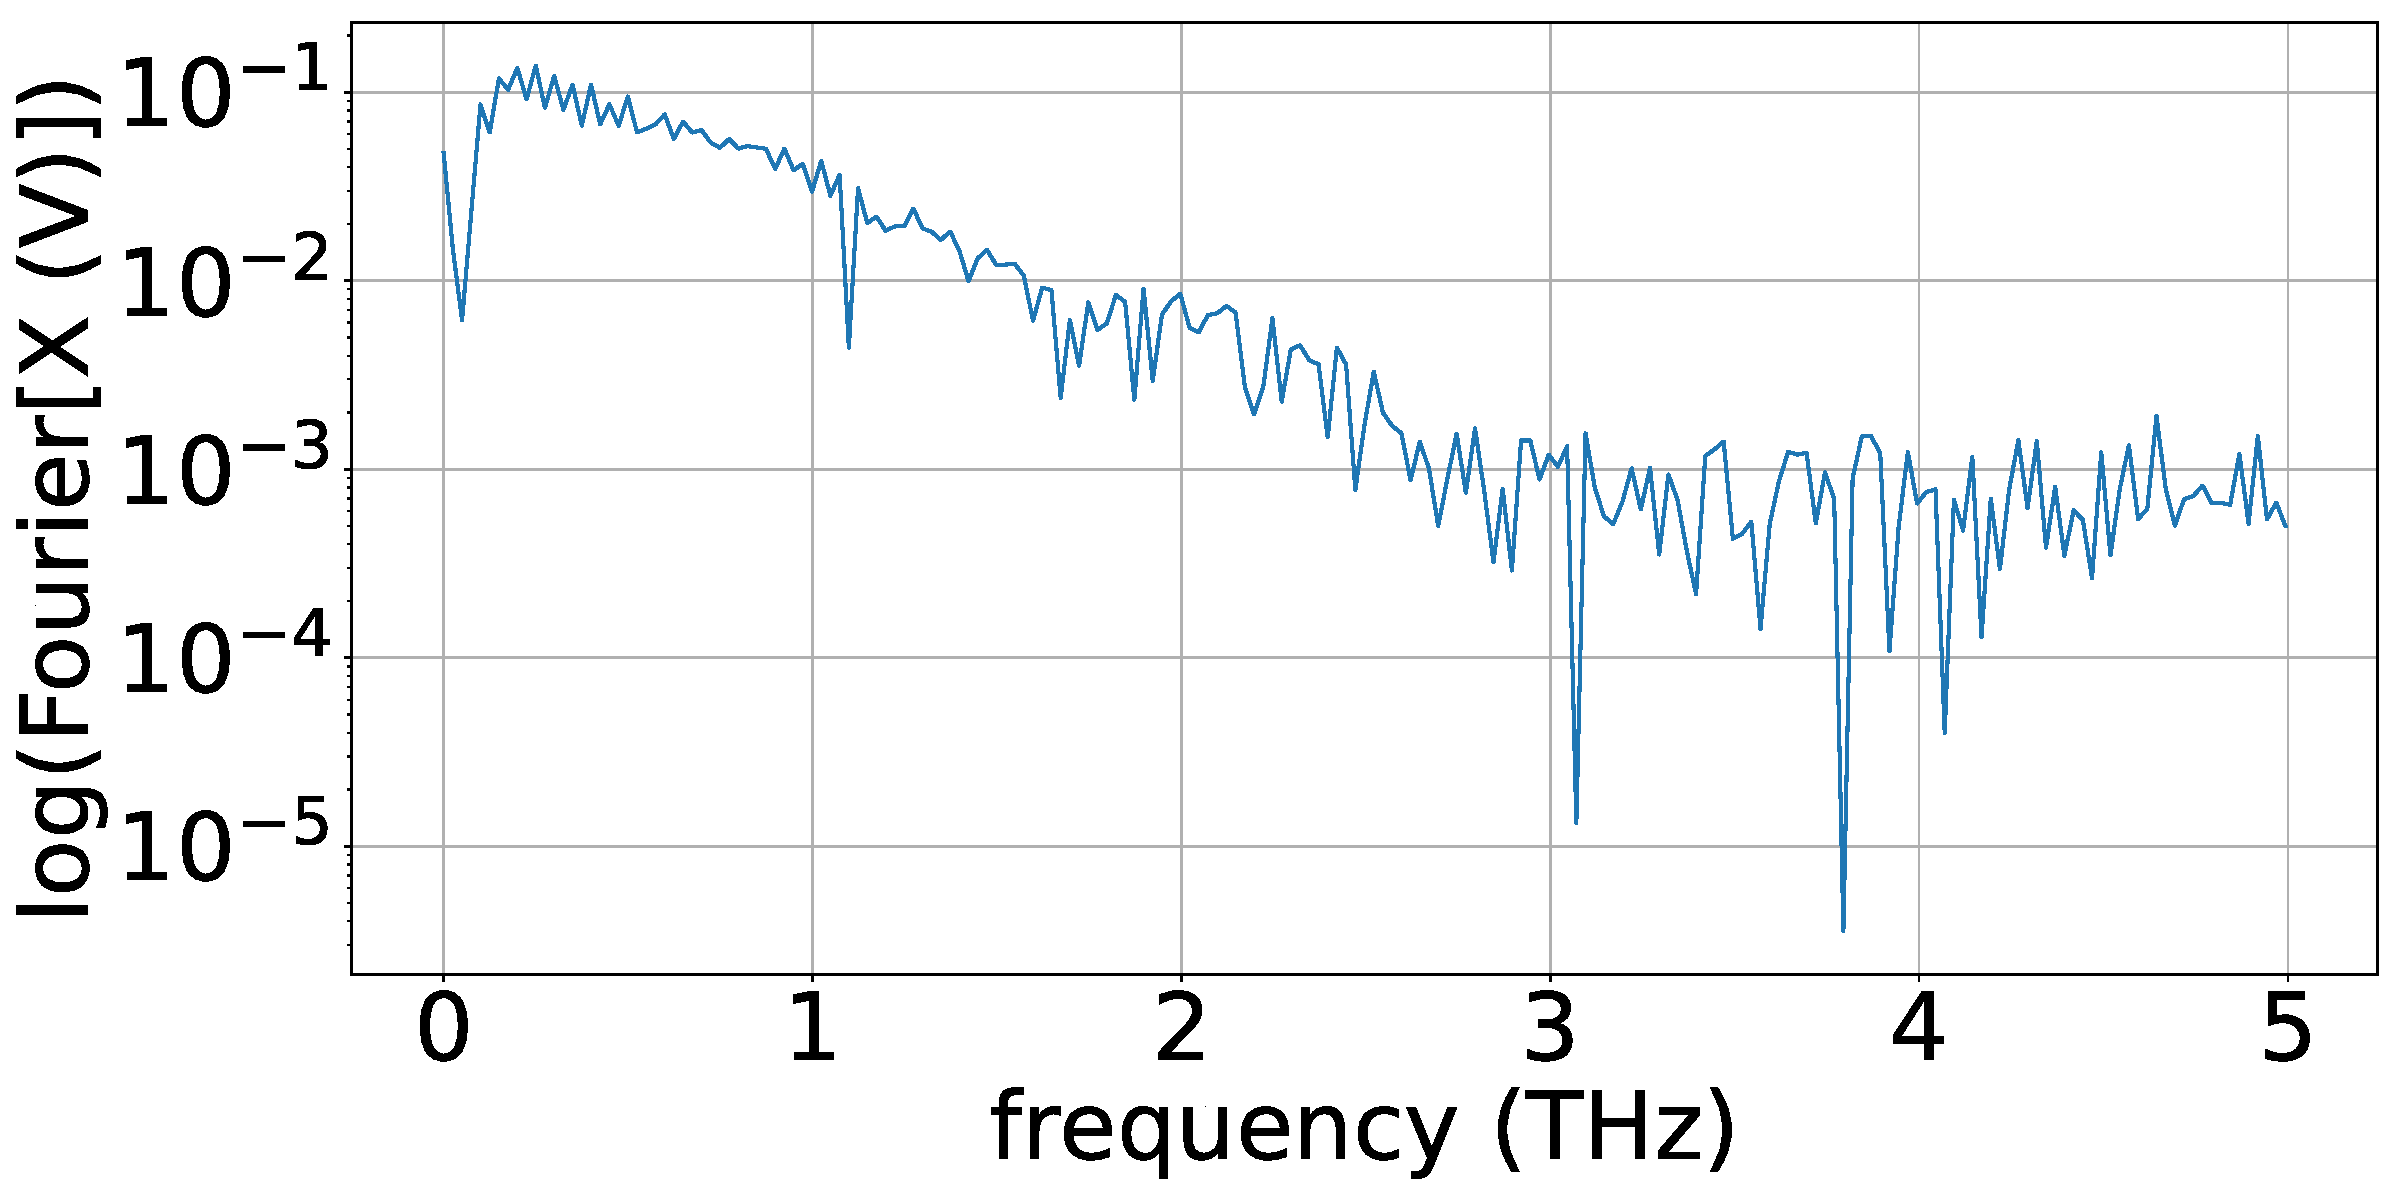
\includegraphics[height=0.75cm]{Plots/2_11_30_20normallog(FX).pdf}%
        \caption{Das TU-Logo.}%
        \label{fig:TU}%
    \end{subfigure}%
    \caption{Zwei Logos, Abbildung \subref{fig:TU}: Das TU-Logo.}%
    \label{fig:logos}%
\end{figure}%
\subsection{Fluence measurments}

\subsection{Electric field measurments}


\section{Gallium phosphide}
\subsection{Fluence measurments}
\subsection{Electric field measurments}


\section{Comparisson}